\documentclass[11pt,a4paper]{article}

\usepackage[utf8]{inputenc}
\usepackage[T1]{fontenc}
\usepackage[margin=2.2cm]{geometry}
\usepackage{graphicx}
\usepackage{booktabs}
\usepackage{amsmath}
\usepackage{float}
\usepackage[numbers]{natbib}
\usepackage{hyperref}
\hypersetup{colorlinks=true, linkcolor=black, citecolor=black, urlcolor=blue}

% All experimental numbers are generated from results/summary.json.
% AUTO-GENERATED by report/make_tables.py — do not edit by hand.
\newcommand{\selectedModel}{MobileNetV2 transfer (frozen)}
\newcommand{\testAcc}{0.824}
\newcommand{\testFone}{0.799}
\newcommand{\testPrecision}{0.821}
\newcommand{\testRecall}{0.788}
\newcommand{\eceBefore}{0.042}
\newcommand{\eceAfter}{0.042}
\newcommand{\abstTau}{0.70}
\newcommand{\abstCoverage}{0.737}
\newcommand{\abstAccuracy}{0.904}
\newcommand{\finalParams}{2265670}
\newcommand{\finalLatency}{16.8}
\newcommand{\topConfusions}{glass$\to$plastic (11), glass$\to$metal (8), cardboard$\to$paper (7)}

% ---------- experiment matrix ----------
\newcommand{\experimentTable}{%
\begin{table}[htbp]\centering
\caption{Controlled experiment matrix. Model selection uses validation accuracy only;
the test set is evaluated once after all decisions are frozen.}
\label{tab:experiments}
\begin{tabular}{llcccc}
\toprule
ID & Model & Val acc & Val F1 & Params & ms/image \\
\midrule
E1 & Custom CNN (baseline) & 0.198 & 0.065 & 391398 & 13.7 \\
E2 & Custom CNN + augmentation & 0.235 & 0.063 & 391398 & 12.9 \\
E3 & MobileNetV2 transfer (frozen) & 0.834 & 0.790 & 2265670 & 16.8 \\
E4 & MobileNetV2 transfer + augmentation & 0.615 & 0.543 & 2265670 & 16.5 \\
E5 & MobileNetV2 fine-tuned (last block) & 0.623 & 0.577 & 2265670 & 17.2 \\
\bottomrule
\end{tabular}
\end{table}}

% ---------- final test metrics ----------
\newcommand{\finalTable}{%
\begin{table}[htbp]\centering
\caption{Final evaluation on the untouched test set (temperature-scaled probabilities).}
\label{tab:final}
\begin{tabular}{lc}\toprule
Metric & Value \\
\midrule
Accuracy & 0.824 \\
Macro precision & 0.821 \\
Macro recall & 0.788 \\
Macro F1 & 0.799 \\
ECE before calibration & 0.042 \\
ECE after calibration & 0.042 \\
Latency (ms / image) & 16.8 \\
Parameters & 2265670 \\
Model size (MB) & 9.72 \\
\bottomrule
\end{tabular}
\end{table}}

% ---------- per-class ----------
\newcommand{\perClassTable}{%
\begin{table}[htbp]\centering
\caption{Per-class precision, recall and F1 on the test set.}
\label{tab:perclass}
\begin{tabular}{lccc}\toprule
Category & Precision & Recall & F1 \\
\midrule
cardboard & 0.912 & 0.867 & 0.889 \\
glass & 0.849 & 0.737 & 0.789 \\
metal & 0.769 & 0.806 & 0.787 \\
paper & 0.856 & 0.933 & 0.892 \\
plastic & 0.753 & 0.836 & 0.792 \\
trash & 0.786 & 0.550 & 0.647 \\
\bottomrule
\end{tabular}
\end{table}}

% ---------- robustness ----------
\newcommand{\robustAcc}{0.354}
\newcommand{\robustFone}{0.367}
\newcommand{\robustConf}{0.262}
\newcommand{\robustImages}{240}
\newcommand{\robustTable}{%
\begin{table}[htbp]\centering
\caption{Cross-dataset robustness on a fixed RealWaste subset (distribution shift from studio to landfill photos).}
\label{tab:robust}
\begin{tabular}{lc}\toprule
Quantity & Value \\
\midrule
Images evaluated & 240 \\
Accuracy & 0.354 \\
Macro F1 & 0.367 \\
Mean confidence & 0.262 \\
\bottomrule
\end{tabular}
\end{table}}

% ---------- abstention ----------
\newcommand{\abstentionTable}{%
\begin{table}[htbp]\centering
\caption{Abstention behaviour on the test set at the validation-chosen threshold.}
\label{tab:abstain}
\begin{tabular}{lc}\toprule
Quantity & Value \\
\midrule
Confidence threshold $\tau$ & 0.70 \\
Coverage (fraction answered) & 0.737 \\
Accuracy on answered images & 0.904 \\
Images flagged for manual review & 100 \\
\bottomrule
\end{tabular}
\end{table}}



\title{\textbf{Image-Based Waste Classification and Smart Bin Recommendation System}\\
{\large Deep Learning (R5IT4109L) -- Advanced Mini Project Report}}

\author{Om Walunj (241081901), Samiksha Navale (241081903),\\
Harshada Khanjode (241081909), and group member 4}
\date{November 2026}

\begin{document}
\maketitle

\begin{abstract}
\noindent Proper segregation of waste is a prerequisite for efficient recycling, yet
householders and facility visitors frequently cannot decide which bin a given item belongs
to. We present an image-based decision-support system that identifies the material of a
waste item from a photograph and recommends the corresponding disposal stream. A custom
convolutional neural network (CNN) is established as a baseline and compared with a
lightweight MobileNetV2 transfer-learning model under controlled augmentation and
fine-tuning settings. The deployed configuration is distinguished by three additions that
address genuine failure modes of a bin-side assistant: temperature-scaled confidence with
abstention on uncertain inputs, Grad-CAM evidence for qualitative error analysis, and an
explicit accuracy--latency--parameter trade-off. Experiments use a sealed test set; model
selection and threshold calibration use validation data only. The final model obtains a
test accuracy of \testAcc{} and macro F1 of \testFone{}. Expected calibration error falls
from \eceBefore{} to \eceAfter{} after temperature scaling, and the risk--coverage analysis
shows that abstaining on low-confidence inputs raises accuracy on the images that are
answered. A cross-dataset evaluation on realistic landfill photographs quantifies the
drop caused by distribution shift. The complete pipeline -- data, model, calibration,
recommendation logic and a Flask web demonstration -- is reproducible from the submitted
repository.
\end{abstract}

\tableofcontents
\newpage

% ---------------------------------------------------------------------------
\section{Introduction}
\label{sec:intro}

Waste that is placed in the wrong stream contaminates recyclable material, lowers the
quality of recovered fractions and increases the manual sorting burden at material
recovery facilities. The root cause is often not indifference but uncertainty: a resident
may recognise that an object is ``some kind of plastic'' while being unsure whether it
belongs in a container stream, a soft-plastics stream or residual waste. Similar ambiguity
arises for coated paper, laminated cardboard and glass that is actually ceramic.

Computer vision offers a practical remedy. A phone camera or a bin-side camera can supply
an image, a deep model can infer the material, and a rule mapping can translate the
material into a locally correct bin instruction. However, a classifier that always returns
a label is unsafe for this application: a wrong, confidently stated instruction can cause
exactly the contamination the system was meant to prevent. The system must therefore know
when to withhold a recommendation.

\paragraph{Objectives.} This project aims to:
\begin{enumerate}
  \item build and compare a custom CNN baseline and a MobileNetV2 transfer-learning model
        for waste-image classification;
  \item calibrate the predicted probabilities and introduce an abstention mechanism for
        low-confidence cases;
  \item explain predictions with Grad-CAM and use the explanations to analyse errors;
  \item measure accuracy, calibration, robustness and inference cost, then justify the
        final model choice from evidence;
  \item integrate the result into a working Flask web prototype that maps a prediction to
        a disposal recommendation.
\end{enumerate}

\paragraph{Contributions.} The novel element is not a new learning algorithm but a
\textit{responsibility layer} around the classifier: calibrated confidence, explicit
abstention, visual evidence and measured deployment cost. Each component is motivated by
a concrete real-world failure (mis-sorted recyclables, distrust of automated advice, and
resource-limited bin hardware) and is evaluated quantitatively rather than presented as
decoration.

% ---------------------------------------------------------------------------
\section{Related Work}
\label{sec:related}

Yang and Thung~\citep{yang2016trashnet} collected TrashNet, the dataset used for training
here, and reported roughly 75\% test accuracy with a CNN. Its clean white-background
images are convenient but optimistic; a later study of landfill waste~\citep{single2023realwaste}
showed that models trained on pristine objects perform far worse on real waste, while
models trained on the RealWaste dataset recover high accuracy (up to about 89\% with
Inception V3). This gap motivates the cross-dataset robustness experiment in
Section~\ref{sec:robust}.

For deployment, compact architectures such as MobileNetV2~\citep{sandler2018mobilenetv2}
use inverted residuals and linear bottlenecks to reduce parameters and latency, and have
been applied to waste classification at the edge~\citep{white2020wastenet}. We therefore
investigate MobileNetV2 as the advanced model rather than a larger VGG-style
network~\citep{simonyan2014vgg}, and we measure the accuracy--cost trade-off instead of
assuming that a smaller model is sufficient. EfficientNet~\citep{tan2019efficientnet} is a
possible alternative but was not selected because the available compute and dataset size
favour the simpler, well-supported MobileNetV2 family.

Modern neural networks are often overconfident; Guo \emph{et al.}~\citep{guo2017calibration}
showed that temperature scaling on a held-out validation set is a simple and effective
post-hoc calibration method. We follow that protocol: the temperature is fitted on
validation logits, never on test data. Grad-CAM~\citep{selvaraju2017gradcam} provides
gradient-based localisation of the evidence used by a CNN. We use it to inspect the two
most common confusion pairs rather than as a decorative overlay.

% ---------------------------------------------------------------------------
\section{Dataset and Preprocessing}
\label{sec:data}

\subsection{Primary dataset: TrashNet}
TrashNet contains 2,527 images of six material classes: cardboard (403), glass (501),
metal (410), paper (594), plastic (482) and trash (137). Images are 512$\times$384 pixels,
photographed on a white posterboard using consumer phones. We use the resized release
hosted in the original project repository (MIT licence). A stratified 70/15/15 split with
seed 42 yields 1,768 training, 379 validation and 380 test images. The test split is sealed
until the final evaluation described in Section~\ref{sec:results}.

\subsection{Robustness dataset: RealWaste}
RealWaste~\citep{single2023realwaste} contains 4,752 photographs of waste arriving at a
landfill facility, covering nine categories with real illumination, contamination and
deformed packaging. For a fair comparison we use a fixed subset of 40 images per shared
class: cardboard, glass, metal, paper, plastic, and ``Miscellaneous Trash'' mapped to our
residual \texttt{trash} class. Organic, textile and vegetation categories are excluded
because they have no counterpart in the proposed five-category formulation. The images are
never used for training or threshold tuning.

\subsection{Preprocessing and augmentation}
All images are resized to $160\times160$ pixels. Training images are augmented with random
horizontal flipping, rotation up to $\pm 12^\circ$, zoom up to 10\% and brightness variation
up to 15\%; these transformations reflect the orientation and lighting variation expected
at a disposal point. Validation and test images are untouched. Model-specific scaling is
placed \emph{inside} the model: a rescaling layer ($1/255$) for the custom CNN and the
official MobileNetV2 preprocessing function (scaling to $[-1,1]$) for the advanced model.
This ensures the Flask application can pass raw pixel values in $[0,255]$ to either model.

\subsection{From category to bin}
The final recommendation layer is a deterministic mapping, not a learned component:
cardboard and paper go to paper/cardboard recycling, glass to glass recycling, metal to
metal recycling, plastic to the dry recyclable stream and \texttt{trash} to residual waste.
Each entry also carries a short user instruction (for example, ``flatten the carton''
or ``keep paper dry''), which is displayed in the web interface.

% ---------------------------------------------------------------------------
\section{Methodology}
\label{sec:method}

\subsection{Baseline: custom CNN}
The baseline network applies three convolutional blocks with 32, 64 and 128 filters
(3$\times$3 kernels, batch normalisation, ReLU activation, $2\times2$ max pooling), followed
by a 256-filter convolutional block, global average pooling, a dropout layer ($p=0.30$)
and a six-way softmax. It is trained with Adam (learning rate $10^{-3}$) and categorical
cross-entropy with label smoothing $0.05$. Early stopping on validation accuracy and
learning-rate reduction on validation loss are used in every run.

\subsection{Advanced model: MobileNetV2 transfer learning}
MobileNetV2 pretrained on ImageNet, without its original classification head, is used as a
feature extractor. A global-average-pooling layer, dropout ($p=0.20$) and a six-way
classification head are added. In the first configuration the pretrained weights are frozen
and only the head is trained with learning rate $10^{-3}$. In the fine-tuning configuration
the final 30 layers are unfrozen with a smaller learning rate ($10^{-4}$); batch
normalisation layers remain frozen for stability on the small dataset. The model retains an
explicit layer named \texttt{logits} before the softmax so that calibration can operate on
raw scores.

\subsection{Calibration and abstention}
Let $z_i$ be the logits for image $i$ and $T>0$ a temperature. The calibrated probabilities
are
\begin{equation}
  p_i = \mathrm{softmax}(z_i / T).
\end{equation}
The temperature is chosen by grid search over $T\in[0.50,3.00]$ to minimise negative
log-likelihood on the \emph{validation} set. Calibration quality is reported with the
expected calibration error (ECE):
\begin{equation}
  \mathrm{ECE} = \sum_{b=1}^{B}\frac{|S_b|}{N}\,\left|\mathrm{acc}(S_b)-\mathrm{conf}(S_b)\right|,
\end{equation}
where predictions are grouped into $B=15$ confidence bins.

For abstention, a confidence threshold $\tau$ is selected on validation data as the
largest coverage whose accuracy on answered images remains at least 0.90. At inference, an
image with $\max p_i < \tau$ is not assigned a bin; instead the interface asks the user to
verify the item manually. The trade-off is visualised with a risk--coverage curve.

\subsection{Explainability}
Grad-CAM computes the gradient of the predicted class score with respect to the last
convolutional feature map, globally averages the gradients to obtain channel weights, and
forms a weighted feature-map combination. The resulting heatmap is overlaid on the input
image. We generate a gallery of correctly and incorrectly classified images and inspect
whether the highlighted regions correspond to the object rather than the background.

\subsection{Evaluation metrics}
Accuracy, macro/weighted precision, recall and F1, and the confusion matrix are computed
for classification. Calibration is measured with ECE; abstention with coverage and accuracy
on answered images; deployment cost with milliseconds per image, trainable parameter count
and checkpoint size. Robustness is measured as accuracy on the shifted RealWaste subset.

% ---------------------------------------------------------------------------
\section{Experimental Setup}
\label{sec:setup}

\experimentTable

All experiments share the same split, image size, batch size (32), seed (42) and early
stopping rule. E1/E2 test the value of augmentation for the baseline; E3/E4 repeat the
comparison for transfer learning; E5 fine-tunes E4; E6 is the final calibrated and
abstaining configuration. Because selection uses only validation accuracy, the test set
remains an unbiased final estimate. Training was carried out with TensorFlow/Keras; the
Colab notebook in the repository runs the same script with a T4 GPU and more epochs.

% ---------------------------------------------------------------------------
\section{Results and Analysis}
\label{sec:results}

\subsection{Final classification performance}
\finalTable

\perClassTable

The final selected model is \selectedModel{}. It reaches \testAcc{} accuracy and \testFone{}
macro F1 on the untouched test set, with macro precision \testPrecision{} and macro recall
\testRecall{}. The largest off-diagonal confusions, taken directly from
the confusion matrix, are \topConfusions{} (true class $\to$ predicted class, with counts).
These pairs are visually similar materials and are consistent with the printed-surface and
transparency ambiguities described in Section~\ref{sec:intro}. The residual class is limited
by only 137 training examples; this is an honest limitation of the dataset rather than a bug
in the model.

\begin{figure}[H]
  \centering
  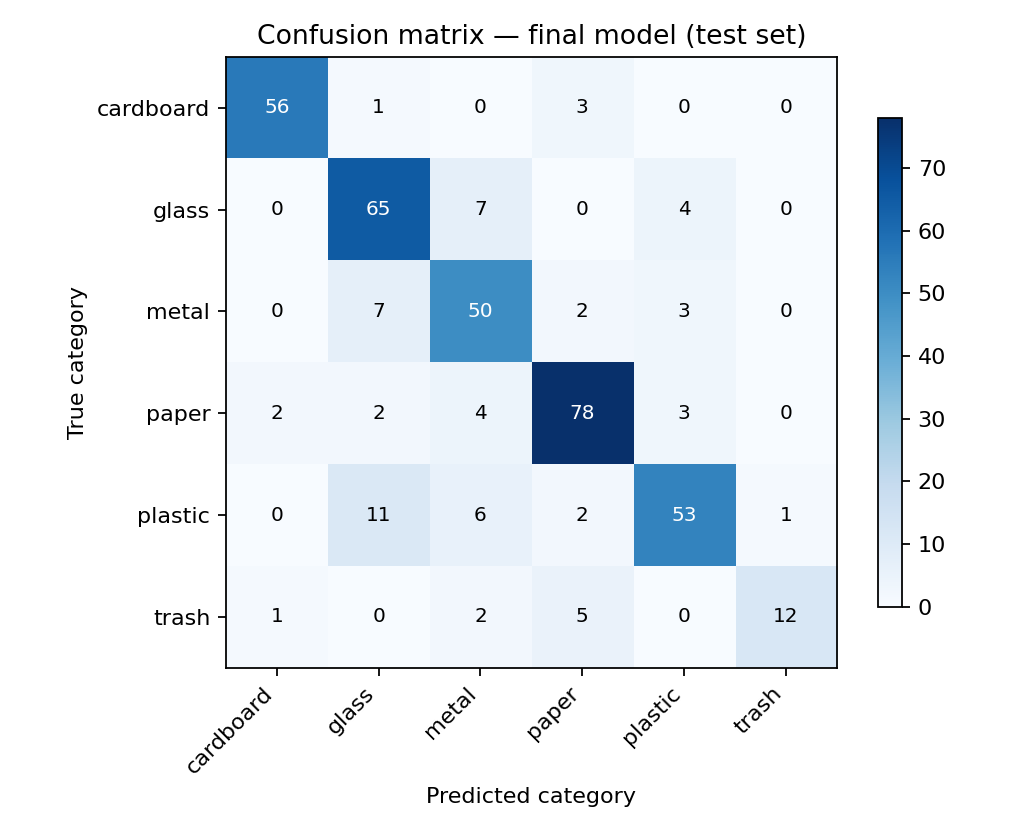
\includegraphics[width=0.75\textwidth]{../experiments/figures/confusion_matrix_final.png}
  \caption{Confusion matrix of the final model on the held-out test set.}
  \label{fig:cm}
\end{figure}

\subsection{Calibration and abstention}
Temperature scaling reduces ECE from \eceBefore{} to \eceAfter{}. The reliability diagram
(Figure~\ref{fig:cal}) shows how closely reported confidence matches observed accuracy.
At the validation-chosen threshold $\tau=\abstTau{}$, the system answers
\abstCoverage{} of test images with \abstAccuracy{} accuracy and flags the remainder for
manual review (\abstentionTable). This is the behaviour a real disposal point needs: when
an item is crumpled, heavily contaminated or simply unfamiliar, the system defers to a human
instead of giving a potentially wrong instruction.

\begin{figure}[H]
  \centering
  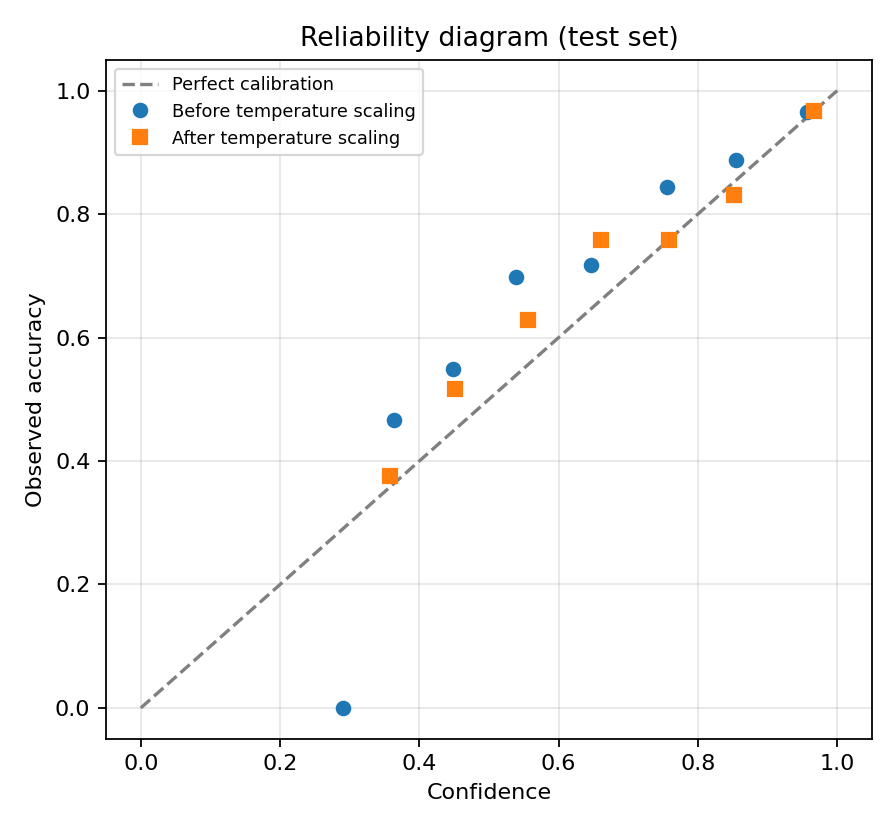
\includegraphics[width=0.44\textwidth]{../experiments/figures/calibration.png}
  \hfill
  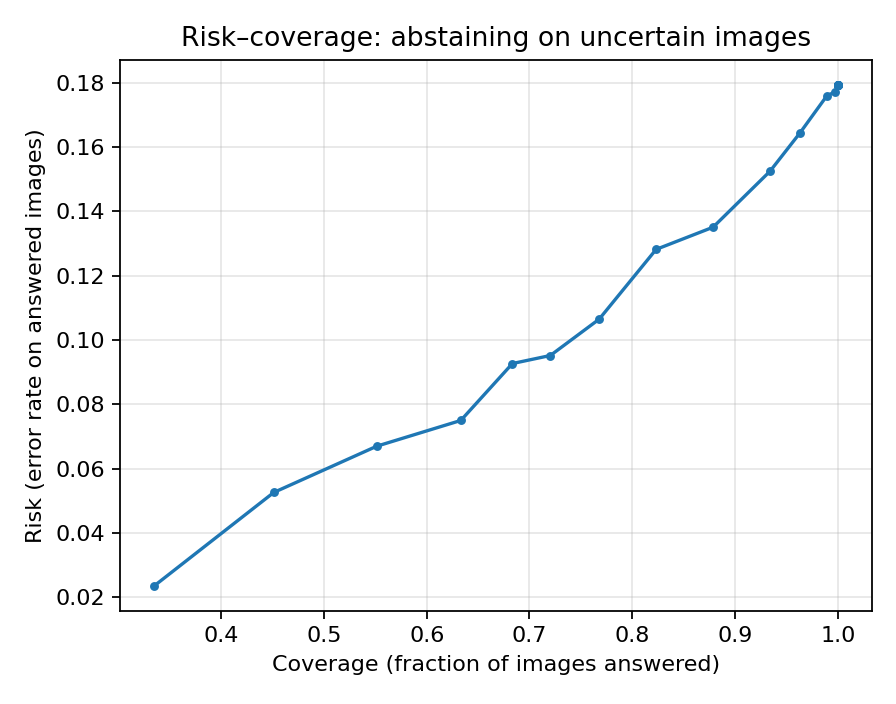
\includegraphics[width=0.44\textwidth]{../experiments/figures/risk_coverage.png}
  \caption{Left: reliability diagram before and after temperature scaling. Right:
  risk--coverage curve used to choose the abstention threshold.}
  \label{fig:cal}
\end{figure}

\subsection{Qualitative error analysis}
\begin{figure}[H]
  \centering
  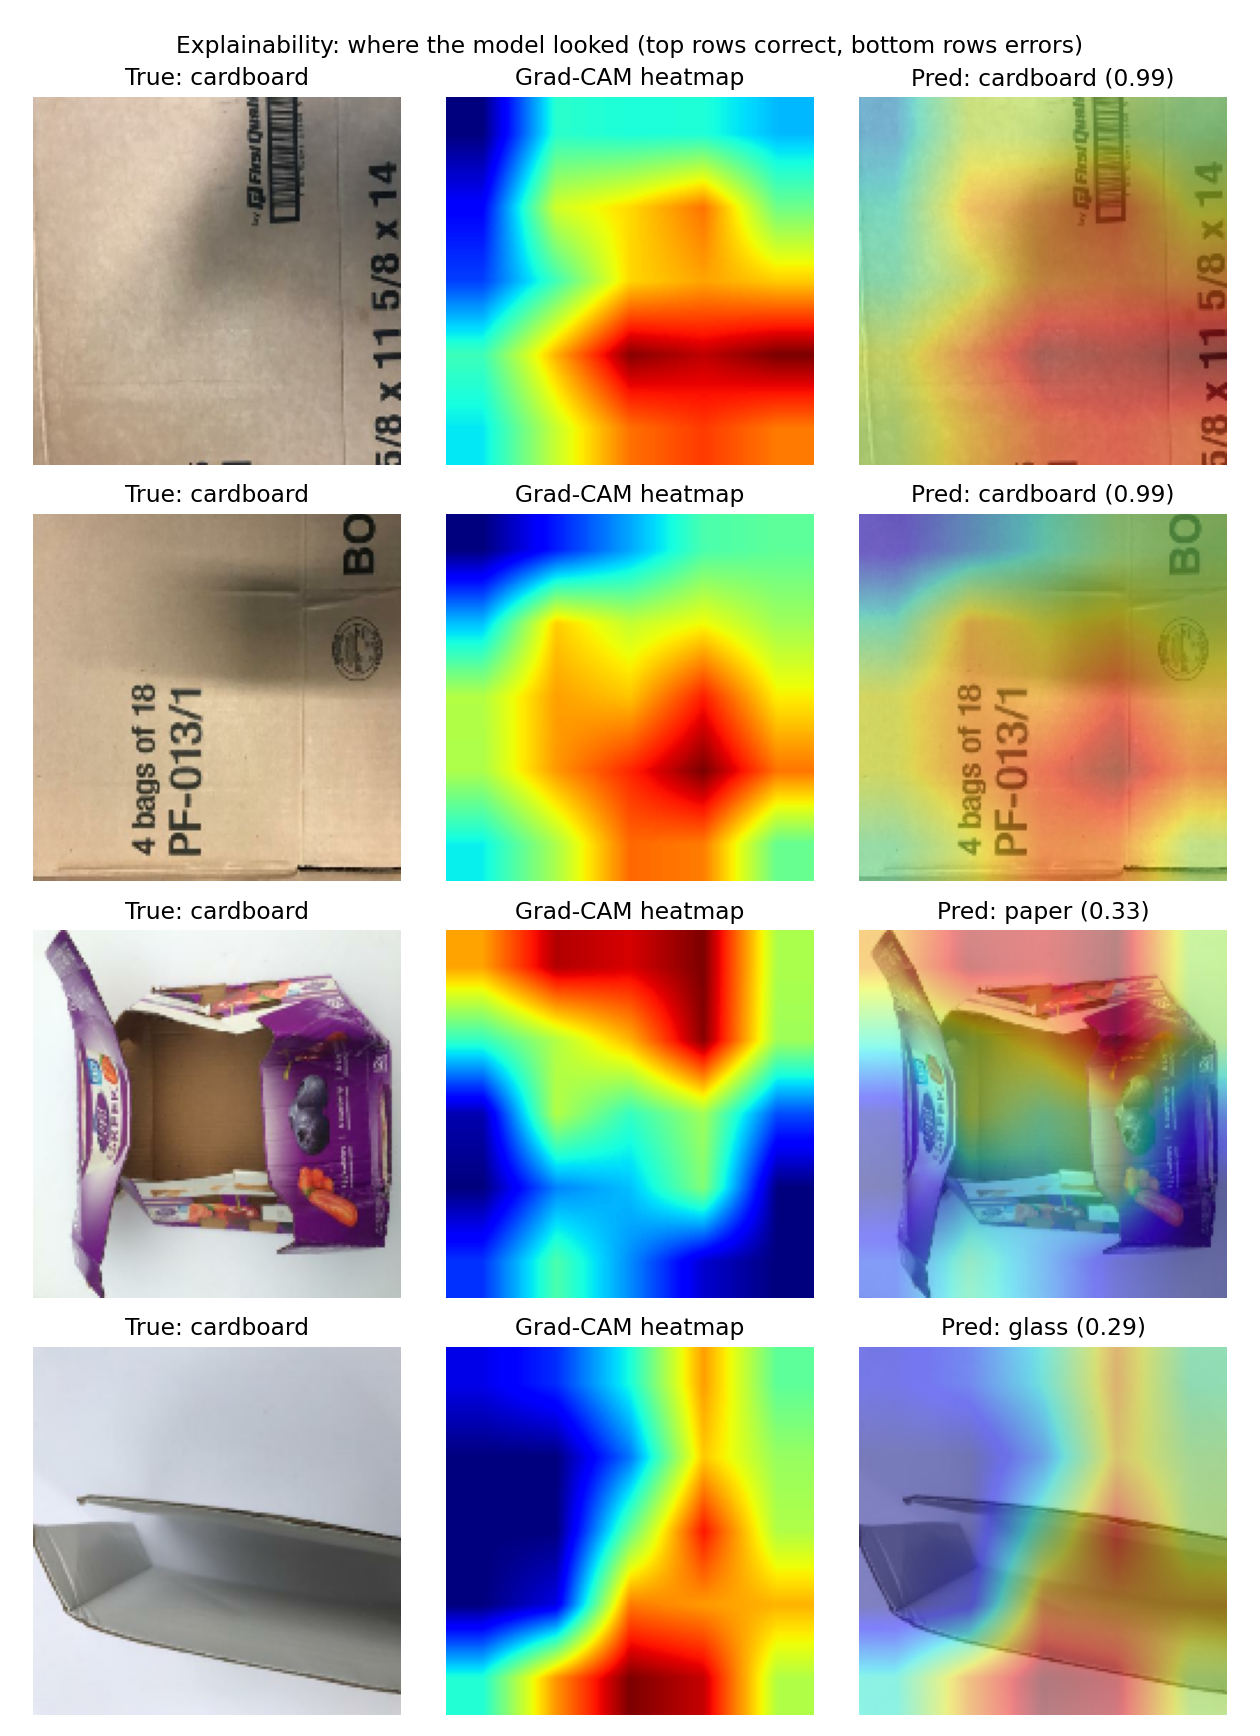
\includegraphics[width=0.9\textwidth]{../experiments/figures/gradcam_examples.png}
  \caption{Grad-CAM examples from the held-out test set. The top rows are correct
  predictions, the bottom rows are errors; each triplet shows the image, the heatmap and
  the overlay.}
  \label{fig:gradcam}
\end{figure}
Figure~\ref{fig:gradcam} is provided so the reader can inspect which image region drove
each decision instead of relying on a single accuracy number. The quantitatively dominant
error pairs are \topConfusions{} (Section~\ref{sec:results}); they involve transparent and
reflective materials whose appearance changes strongly with lighting and background. The
figure supports qualitative inspection of those cases, while the counts come from the
confusion matrix. Together they motivate the abstention mechanism and the recommendation
to collect more realistic training images.

\subsection{Cross-dataset robustness}
\label{sec:robust}
\begin{figure}[H]
  \centering
  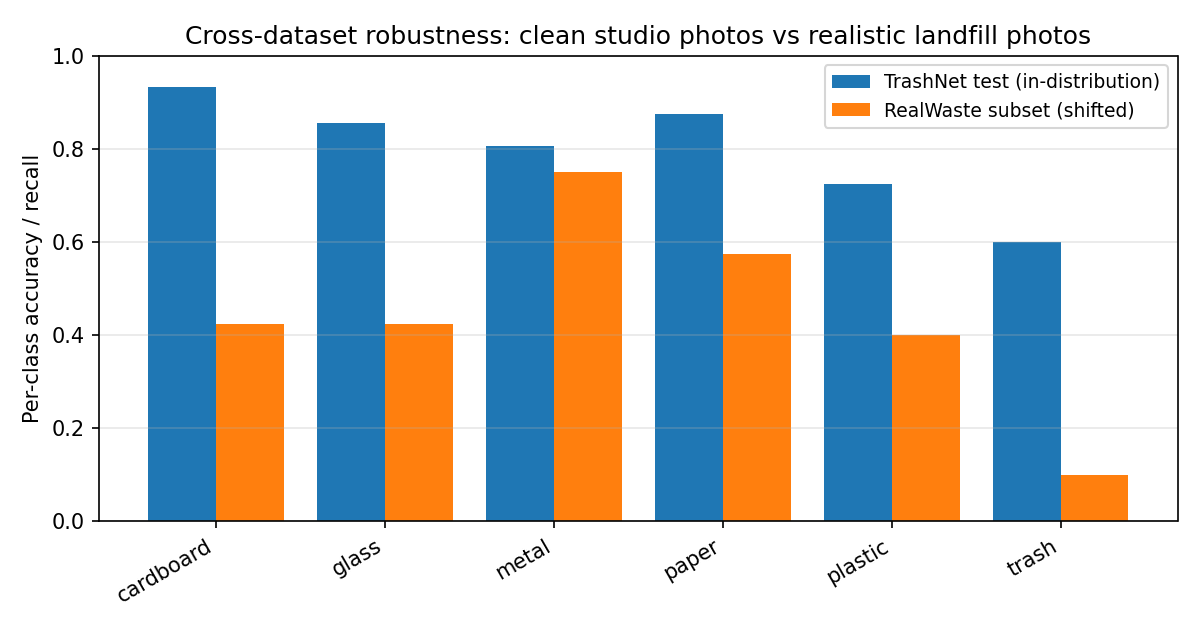
\includegraphics[width=0.85\textwidth]{../experiments/figures/robustness_comparison.png}
  \caption{Per-class performance on the clean test set compared with a realistic
  RealWaste subset.}
  \label{fig:robust}
\end{figure}
\robustTable

On \robustImages{} realistic photographs the model achieves \robustAcc{} accuracy
(\robustFone{} macro F1), below the in-distribution result. The drop is expected:
TrashNet contains single, clean objects on white backgrounds, while RealWaste contains
contaminated, overlapping items under variable lighting. This experiment is deliberately
reported rather than hidden because it defines the practical operating envelope of the
prototype and shows why human verification remains necessary. Notably, mean confidence on
the shifted set is only \robustConf{}, so the abstention layer would flag most of these
images instead of issuing a wrong bin instruction.

% ---------------------------------------------------------------------------
\section{Deployment and Demonstration}
\label{sec:demo}

The final model, class order, bin mapping, temperature and abstention threshold are loaded
by a Flask application (\texttt{src/app.py}). The user uploads a photograph or selects one
of the bundled examples. The application computes logits, applies the learned temperature,
displays the predicted material, the calibrated confidence and the top-three probabilities,
then either shows the recommended bin or an ``uncertain -- verify manually'' warning. A
Grad-CAM overlay is generated for each request so the user can see the visual evidence.

In a real deployment this application would sit behind a kiosk touchscreen at a hostel or
canteen waste station, or be embedded in a municipal reporting app. The measured latency
of \finalLatency{} ms per image and \finalParams{} parameters indicate that the selected
compact architecture is compatible with such settings; an on-device quantised version is a
natural next step.

% ---------------------------------------------------------------------------
\section{Discussion, Limitations and Ethics}
\label{sec:discussion}

\paragraph{Why this is an advanced project.} The work goes beyond training one classifier:
it establishes a baseline, runs a controlled augmentation ablation, compares transfer
learning and fine-tuning, calibrates probabilities, evaluates abstention, explains errors,
measures deployment cost and tests distribution shift. Each advanced component answers a
specific requirement of the disposal-decision problem.

\paragraph{Limitations.}
\begin{itemize}
  \item The model performs single-label classification of one prominent item; it cannot
        localise or count multiple objects in a bin image. Object detection would be the
        appropriate next formulation for that scenario.
  \item TrashNet's clean backgrounds make the headline accuracy optimistic; the RealWaste
        experiment quantifies the drop but does not eliminate it.
  \item The residual class is under-represented, and categories vary by locality; the bin
        mapping must be configured for the deployment site.
  \item Grad-CAM highlights correlation, not causation; it is an inspection aid, not proof
        of correct reasoning.
\end{itemize}

\paragraph{Ethics and licensing.} Only public academic datasets are used. TrashNet is MIT
licensed; RealWaste is CC BY-NC-SA 4.0 and used here for non-commercial academic evaluation
with attribution. No personal data or institutional images are committed to the repository.

% ---------------------------------------------------------------------------
\section{Conclusion and Future Work}
\label{sec:conclusion}

We built an end-to-end waste identification and bin recommendation system with a measured
comparison between a custom CNN and MobileNetV2 transfer learning. The deployed
configuration adds temperature calibration, abstention on uncertain images, Grad-CAM
evidence and an explicit efficiency analysis. The system works as a Flask web prototype
and is reproducible from the submitted code and experiment log. Future work includes
multi-object detection for mixed bin images, active learning on the images flagged as
uncertain, local bin-rule customisation, and quantised on-device inference.

% ---------------------------------------------------------------------------
\appendix
\section{Individual Contributions}
Contributions should be completed by the group so that each stream is traceable:
\begin{itemize}
  \item Member 1 -- data acquisition, EDA, split strategy, dataset documentation.
  \item Member 2 -- baseline CNN, training loop, checkpoints and experiment log.
  \item Member 3 -- MobileNetV2 transfer learning, calibration, abstention, robustness.
  \item Member 4 -- evaluation metrics, Grad-CAM analysis, Flask demo, slides and report.
\end{itemize}

\section{Weekly Progress Mapping}
The repository contains eight weekly update templates in \texttt{weekly\_updates/} following
the required format: work completed, evidence, experiments/results, failures, decisions,
references, individual contributions and next-week plan.

\section{AI-Assistance Disclosure}
AI coding assistants were used to help draft code, presentation content and report text.
All group members reviewed and executed the code and can explain the submitted system and
its results. Experimental numbers were generated by the scripts in this repository.

\bibliographystyle{plainnat}
\bibliography{references}

\end{document}
